\chapter{Teakwood System }

\section{Overview}
Structurally, like most websites, Teakwood system has a three-layer layout: frontend, backend, and database. Becuase Teakwood uses computing servers to run jobs, so the eco Teakwood system actually has four layers; the up mentioned three plus a computing layer. the below figure shows how is the four-layer structure like:\\

\begin{figure}[htb]
\centering
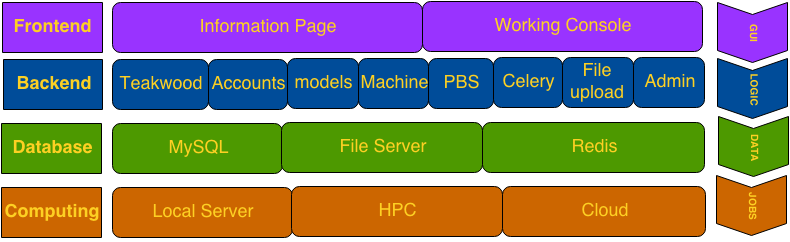
\includegraphics[scale=0.5]{./system_structure} 
% e.g. insert ./image for image.png in the working directory, adjust scale as necessary
\caption{Teakwood System Overview}
\label{fig:label} % insert suitable label, this is used to refer to a fig from within the text as shown above
\end{figure}

On the above figure, we can see the four straight layers bottom-up. Each layer from left to right: the left part is the layer name; the middle part is the layer content; and the right part is the layer reality. Let's go through these layers one by one.

\section{Frontend}
The frontend is a visible GUI that user interact with. Basically all what we see in the Teakwood website can be called the "frontend", that includes the HTML files, Functional butthons, the pictures, etc.  For neat purpose, Teakwood separated the frontend into two parts: the \textbf{information pages} and the \textbf{working console}. See below:

\begin{figure}[htb]
\centering
%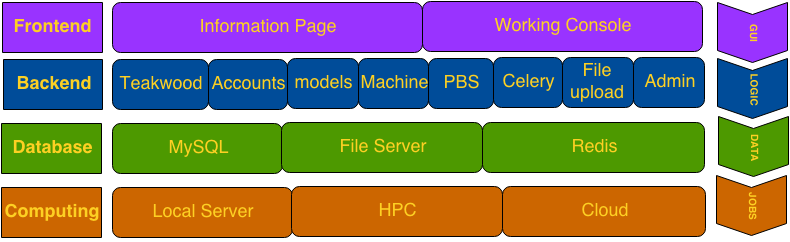
\includegraphics[scale=0.5]{./system_structure} 
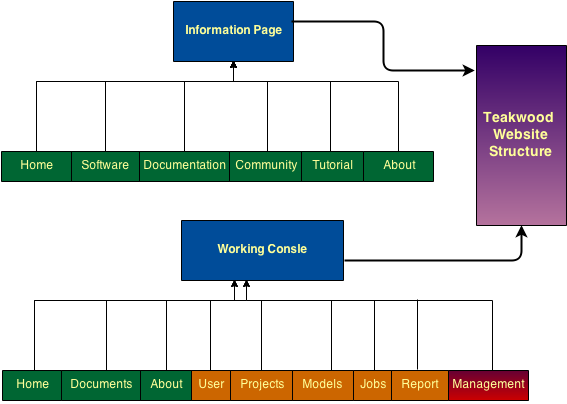
\includegraphics[scale=0.6]{./website_structure} % e.g. insert ./image for image.png in the working directory, adjust scale as necessary
\caption{Website Strucutre}
\label{fig:label} % insert suitable label, this is used to refer to a fig from within the text as shown above
\end{figure}

The \textbf{information pages} introduces you all the general information about Teakwood, including:\\

$\bullet$ What is Teakwood?\\
$\bullet$ What can Teakwood do?\\
$\bullet$ How to install Teakwood?\\
$\bullet$ How to use Teakwood?\\
$\bullet$ The user manual.\\
$\bullet$ Video tutorial.\\
$\bullet$ Teakwood forum.\\


The \textbf{working console} is the working place you actually tango with your project. The functional buttons will guide you to different web pages for different purpose.\\
Let me explain these functional buttons one by one.\\

$\bullet$ \textbf{Home}: Directs you to the homepage.\\
$\bullet$ \textbf{Documents}: Directs you to the user manual.\\
$\bullet$ \textbf{About}: Teakood self introduction.\\
$\bullet$ \textbf{User}: Displays user information.\\
$\bullet$ \textbf{Projects}: Creates projects and provides project overview.\\
$\bullet$ \textbf{Models}: Create models and provides models overview.\\
$\bullet$ \textbf{Jobs}:Creates jobs, overview jobs and job monitoring.\\
$\bullet$ \textbf{Report}:Directs you to the output downloading page.\\
$\bullet$ \textbf{Management}:Access to the admin system.\\


Note the color differences in the bottom layer.\\

$\bullet$ The \textbf{Green}: all visitors can see and manipulate.\\
$\bullet$ The \textbf{orange}: only logging user can see and manipulate.\\
$\bullet$ The \textbf{red}: only superuser can see and manipulate.\\


\section{Backend}
The backend contains all the logical design of data manipulating and HTML producing. In detail, it includes verifying user's request, pulling requested data, generating HTML web page and displaying the web page. Teakwood follows the MVC(Model-View-Controller)design pattern and separated all the system functions in to loose coupled parts, each part is a well wrapped MVC. in Django, it calls "app". These parts will work independently or cooperatively in order to achieve a user's request. We will have a backend chapter to reveal the logic mystery. This section will only  provides a general explanation.

In Teakwood system, there are mainly eight parts(Apps).\\

$\bullet$ \textbf{Teakwood}: controls the frontend presentation.\\
$\bullet$ \textbf{Accounts}: provides the registration logic.\\
$\bullet$ \textbf{Models}: invoke and control the computing models.\\
$\bullet$ \textbf{Machine}: invoke and control the computing resources.\\
$\bullet$ \textbf{PBS}: guides the PBS script generation.\\
$\bullet$ \textbf{File upload}: gathers the input files to buffer for uploading. \\
$\bullet$ \textbf{Admin}: provies an overall control of user and data.\\
$\bullet$ \textbf{Celery}: third party app, handle synchronous processing.\\

\section{Data handling}
Teakwood system handles three types of data: the website data, the computing data and the message queue data. For each type of data Teakwood provides a different storage. see this table:\\
\\   
\begin{table}[h]
\begin{tabular}{lllll}
\cline{1-3}
\multicolumn{1}{|c|}{\textbf{Website data}} & \multicolumn{1}{c|}{\textbf{Computing data}} & \multicolumn{1}{c|}{\textbf{Message queue data}} &  &  \\ \cline{1-3}
\multicolumn{1}{|c|}{\textbf{MySQL}} & \multicolumn{1}{c|}{\textbf{File server}} & \multicolumn{1}{c|}{\textbf{redis server}} &  &  \\ \cline{1-3}
\multicolumn{1}{|c|}{\textbf{Teakwood data}} & \multicolumn{1}{c|}{\textbf{inputs and outputs}} & \multicolumn{1}{c|}{\textbf{Asynchronous handling}} &  &  \\ \cline{1-3}
                                &                                &                                &  & 
\end{tabular}
\end{table}


Teakwood uses MySQL database for storing the website data, e.g. the user account and the project labels.\\
For the computing data, Teakwood periodically synchronize them to the file server for backup and downloading purpose, e.g. input files and the output result.\\
Message queue data is generated when we use Celery to asynchronous process time consuming tasks. Those data are ephemeral, so we simply use a redis server to keep it.\\

\section{Remote Configuration}
Before the first time we can run a job on HPC or cloud, we have set up a connection between Teakwood and the computing servers. In detail, we have four tasks to do:\\

$\bullet$ Establish an password-less ssh login. to the server.\\
$\bullet$ Compile the tools and packages we will use in the remote machine.\\
$\bullet$ Ready all the import path for machine configuration Teakwood.\\
$\bullet$ Configuration Teakwood by the form guidance.\\

After those steps are done, we've successfully "plugged" Teakwood into these remote machines. Now everything we interact with the terminal will migrates to the Teakwood web portal.


%\subsection{<Sub-section title>}

%\subsection{<Sub-section title>}
%some text\cite{citation-2-name-here}, some more text

%Refer figure \ref{fig:label}.


